\subsection{形成性构造}

一个理论的一些特定符号被称为关系性的，而其他的被称为实体性的。每个特定符号都关联一个自然数，称为其权重（实际上通常为2）。

¶ 如果一个组装以τ开头，或以实体符号开头，或者仅由一个字母组成，则称其为第一类组装；否则为第二类组装。

¶ 理论 \(\mathfrak{C}\) 中的一个形成性构造，是满足如下性质的组装序列：序列中的每个组装 A 都满足以下条件之一：

\begin{enumerate}
\def\labelenumi{(\alph{enumi})}
\item
  A 是一个字母。
\item
  在序列中存在一个第二类的组装 B，位于 A 之前，使得 A 是 \(\neg B\) .
\item
  存在两个组装 \(\pmb{B}\) 并且 \(\pmb{C}\) （第二类，相同或不同），位于 \(\pmb{A}\) 之前，使得 \(\pmb{A}\) 是 \(\vee \pmb{BC}\) .
\item
  存在一个第二类的组装 B，位于 A 之前，以及一个字母 x，使得 A 是 \(\tau_{x}(B)\) .
\item
  有一个特定符号 \(s\) ，其权重为 \(n\)\footnote{如上所述，为了发展当今的数学理论，可以将我们的考虑限于权重为 2 的特定符号，从而避免在形成性构造的定义中使用“自然数 n”这一表述。} ，并且属于 \(\mathfrak{C}\) ；还有 \(n\) 个第一类组装 \(A_{1}, A_{2}, \ldots, A_{n}\) ，它们先于 \(A\) 出现，使得 \(A\) 是 \(sA_{1}A_{2} \ldots A_{n}\) 。
\end{enumerate}

¶ 出现在 \(\mathfrak{C}\) 的形成性构造中的第一类（相应地，第二类）组装，称为 \(\mathfrak{C}\) 中的项（相应地，关系）。

示例。*在集合论中，其中 \(\in\) 是权重为2的关系符号，以下组装序列是一个形成性构造：

\pandocbounded{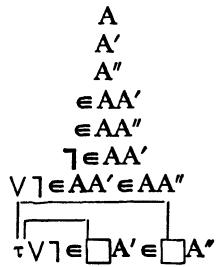
\includegraphics[keepaspectratio]{images/part001_f4a426ee2f8fe397dc0bc6599464a758ff3a832b6925cc474c9242d7de093d2f.jpg}}

因此，第1号示例中给出的组装是集合论中的一个项。*

备注。直观地说，项是表示对象的组装，而关系是表示关于这些对象可以作出的断言的组装。条件（a）意味着字母表示对象。条件（b）意味着如果B是一个断言，那么 \(\neg B\) 称为B的否定，是一个命题（读作：非B）。条件(c)意味着如果B和C是命题， \(\vee BC\) 称为B和C的析取，是一个命题（读作：B或C）；因此 \(\Longrightarrow BC\) 是一个命题（用语言表述为：“非B，或C”，或“B蕴含C”）。条件(d)意味着如果B是一个命题且x是一个字母，那么 \(\tau_{X}(B)\) 是一个对象。让我们将命题B视为表达对象X的一个性质；那么，如果存在一个具有该性质的对象， \(\tau_{X}(B)\) 表示一个具有此性质的特定对象；如果没有， \(\tau_{X}(B)\) 表示一个关于它无法言说的对象。最后，条件(e)意味着如果 \(A_{1}, A_{2}, ..., A_{n}\) 是对象，且s是一个n元关系（或实体）符号，那么 \(sA_{1}A_{2}\ldots A_{n}\) 是关于对象 \(A_{1}, ..., A_{n}\) 的一个命题（相应地，一个依赖于 \(A_{1}, ..., A_{n}\) 的对象).

示例。符号 \(\phi\) , \(\mathbf{N}\) “实数直线”，“该 \(\Gamma\) 函数”， \(f \circ g\) 表示项。符号 \(\pi = \sqrt{2} + \sqrt{3}\) , \(1 \in 2\) ，“每个有限除环都是域”，“\(\zeta(s)\) 的除 \(-2, -4, -6, \ldots\) 之外的零点位于直线上 \(\mathcal{R}(s) = 1/2\)'' 表示关系。符号“3和4”既不表示项，也不表示关系。

关系的初始符号是 \(\vee, \neg\) ，或关系符号。项的初始符号要么是 \(\tau\) 或一个实体性的符号，前提是该项并非由单个字母组成。后一断言源于这样一个事实：项是第一类组装。如果 \(A\) 是一个关系，则 \(A\) 出现在一个形成性构造中，不是字母，且不以 \(\tau\) 开头，因此可能存在三种情况：（1） \(A\) 前面有一个组装 \(B\) 使得 \(A\) 是 \(\neg B\) ; (2) \(A\) 前面有两个组装 \(B\) 和 \(C\) 使得 \(A\) 是 \(\vee BC\) ; (3) \(A\) 前面有组装 \(A_1, A_2, ..., A_n\) 使得 \(A\) 是 \(sA_1A_2 ... A_n\) , \(s\) 作为一个关系符号。

